
\documentclass[11pt]{beamer}
\usetheme{Frankfurt}
\usecolortheme{seahorse}
\usepackage{multirow}
\usepackage{pifont}
\usepackage{bm}
\usepackage{caption}
%\usepackage{subcaption}
\usepackage{url}


\setbeamertemplate{footline}[frame number]
\setbeamertemplate{itemize items}[triangle]
\setbeamertemplate{frametitle}[default][center]




% Symbols
\newcommand{\ra}{\rightarrow}
\newcommand{\ov}{\overline}
\newcommand{\ur}{\underline}
\newcommand{\pr}{\prime}
\newcommand{\tbf}{\textbf}
\newcommand{\omg}{\Omega}
\newcommand{\mc}{\mathcal}
\newcommand{\lt}{\left}
\newcommand{\rt}{\right}
\newcommand{\mb}{\mathbb}
\newcommand{\imp}{\implies}
\newcommand{\dimp}{\Leftrightarrow}
\newcommand{\wh}{\widehat}
\newcommand{\dg}{\mc{D}}


% Sets
\newcommand{\realset}{\mb{R}}
\newcommand{\comprealset}{\mb{\ov{R}}}
\newcommand{\pint}{\mb{Z}_{> 0}}
\newcommand{\nzrl}{\mb{R}_{\geq 0}}
\newcommand{\prl}{\mb{R}_{>0}}
\newcommand{\rl}{\mb{R}}
\newcommand{\fin}{\forall i\in\{1,...,n\}}
\newcommand{\tup}[1]{\{1,...,#1\}}
\newcommand{\seq}[2]{_{#1=1}^#2}
\newcommand{\mCnn}{\mb{M}_{n\times n}(\mb{C})}
\newcommand{\mCmm}{\mb{M}_{m\times m}(\mb{C})}
\newcommand{\mCpn}{\mb{M}_{p\times n}(\mb{C})}
\newcommand{\mCnm}{\mb{M}_{n\times m}(\mb{C})}
\newcommand{\mRnn}{\mb{M}_{n\times n}(\mb{R})}
\newcommand{\mRpn}{\mb{M}_{p\times n}(\mb{R})}
\newcommand{\mRnm}{\mb{M}_{n\times m}(\mb{R})}
\newcommand{\mRno}{{{\mb{R}}}^n_{\geq 0}}
\newcommand{\mRmo}{{{\mb{R}}}^m_{\geq 0}}
\newcommand{\mRo}{\mb{R}_{\geq 0}}
\newcommand{\mRn}{{\mb{R}}^n}
\newcommand{\mRm}{{\mb{R}}^m}
\newcommand{\mCn}{\mb{C}^n}
\newcommand{\mCm}{\mb{C}^m}
\newcommand{\inv}{\mb{GL}_n(\mb{R})}
\newcommand{\id}[1]{\mb{I}_{#1\times #1}}
\newcommand{\mat}[3]{\mb{M}_{#1\times #2}(\mb{#3})}


% matrix operations
\newcommand{\ColumnJoin}[2]{\left[\begin{array}{l}{#1}\\{#2} \end{array}\right]}
\newcommand{\minaffine}[2]{\Lambda^{\min}\lt(#1,#2\rt)}
\newcommand{\maxaffine}[2]{\Lambda^{\max}\lt(#1,#2\rt)}

% local macros
\DeclareMathOperator{\real}{\operatorname{Re}}
\newcommand{\CZ}{\lt(V,c,s\rt)}
\newcommand{\GCZ}{\gcz{V}{c}{s}{W}{l}{u}}
\newcommand{\cz}[3]{\mc{C}\lt(#1,#2,#3\rt)}
\newcommand{\CZO}{\lt(V,0,s\rt)}
\newcommand{\czo}[2]{\mc{Z}\lt(#1,0,#2\rt)}
\newcommand{\trj}[2]{{\bf #1}(#2)}
\newcommand{\IncTcz}[6]{\mc{T}\lt(#1,#2,#3,#4,#5,#6\rt)}
\newcommand{\IncGcz}[6]{\mc{G}\lt(#1,#2,#3,#4,#5,#6\rt)}
\newcommand{\Ptope}[3]{\mc{P}\left(#1,#2,#3\right)}
\newcommand{\gcz}[6]{\mathcal{Z}\lt(#1,#2,#3,#4,#5,#6\rt)}
\newcommand{\sptope}[3]{\mathcal{P}\lt(#1,#2,#3\rt)}
\newcommand{\system}{\mb{H}}
\newcommand{\locationset}{Q}
\newcommand{\edgeset}{E}
\newcommand{\stay}{\gamma}
\newcommand{\linearmapset}{\mc{A}}
\newcommand{\inputset}{U}
\newcommand{\initialset}{\Omega}
\newcommand{\edge}{\sigma}
\newcommand{\loc}{q}
\newcommand{\map}{\linearmapset}
\newcommand{\inp}{\inputset}
\newcommand{\ptemplate}{\mc{K}}
\newcommand{\systrj}[2]{\lt({\bf #1},{\bf #2}\rt)}
\newcommand{\wholenums}{\mb{Z}_\geq 0}
\newcommand{\preloc}[1]{#1_{1}}
\newcommand{\postloc}[1]{#1_{2}}
\newcommand{\upperedgebound}[1]{#1^+}
\newcommand{\loweredgebound}[1]{#1^-}
\newcommand{\reset}[1]{#1_r}
\newcommand{\locationtransition}[1]{R_{#1}}
\newcommand{\edgetransition}[1]{R_{#1}}
\newcommand{\staysptope}[1]{\sptope{\ptemplate\lt(#1\rt)}{\stay^-\lt(#1\rt)}{\stay^+\lt(#1\rt)}}
\newcommand{\guardsptope}[1]{\sptope{\ptemplate\lt(\preloc{#1}\rt)}{\max\lt(\loweredgebound{#1},\stay^-\lt(\preloc{#1}\rt)\rt)}{\min\lt(\upperedgebound{#1},\stay^+\lt(\preloc{#1}\rt) \rt)}}
\newcommand{\hybridset}{\Gamma}
\newcommand{\transfer}[4]{#1#4 = #2\dg\lt(#3\rt)}
\newcommand{\centertransfer}[4]{#1#4 = #3-#2}
\newcommand{\scalebound}[5]{\max_{i=1}^{#4}\lt(\lt(\sum_{j=1}^{#5}\lt|#1\rt|_j\rt)-#3_i+#2_i\rt)}
\newcommand{\pseudoinverse}[1]{#1\lt(#1#1^T\rt)^{-1}}


\title{Augmented Complex Zonotopes for Computing Invariants of Affine Hybrid Systems}
\setbeamercolor{author}{fg=blue}
\author[shortname]{{ \bf \hspace{-1em} Arvind\ Adimoolam~\inst{1}\hspace{1em} Thao\ Dang~\inst{2}}}
\setbeamercolor{institute}{fg=magenta}
\institute{{\bf
\inst{1,2} VERIMAG/ \inst{2}CNRS}\\~Grenoble,France
\begin{figure}
\center
\hspace{2em}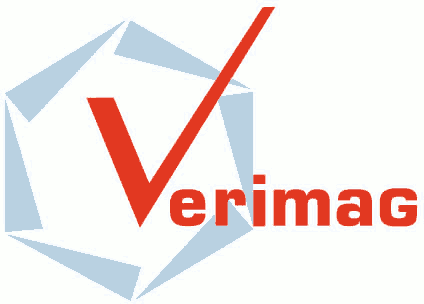
\includegraphics[scale=0.2]{fig/LogoVERIMAG.png}
\end{figure}
}

\date{}

\begin{document}

\maketitle

\begin{frame}{Hybrid behavior of digital control systems}
\textcol{Switch} between \textcol{different control laws}.\\
Eg.  \textcol{Different dynamics} of an engine for \textcol{different gears}.
\begin{figure}
\center
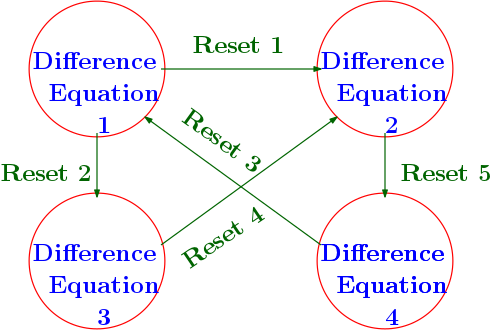
\includegraphics[scale=0.4]{fig/hybrid-model.png}
\end{figure}
\begin{itemize}
\item Difference Equation: $x(t+1)=f_i\lt(x(t),u(t)\rt).$
\item Reset: \vspace{-1.5em}
\begin{align}
\begin{split}
& \text{If}~~x\in S~~\text{(Precondition)}\\
& \text{then}~~x = g_i(x)
\end{split}
\end{align}
\end{itemize}
\end{frame}

\begin{frame}{Affine hybrid system}
\begin{figure}
\center
{\bf Specification}
\end{figure}
\begin{figure}
\center
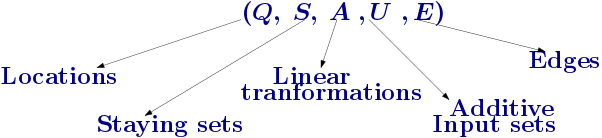
\includegraphics[scale=0.35]{fig/model-spec.png}
\caption*{{\small{\color{darkgray}$\forall q\in Q$, $S_q, U_q$: Polytopic subsets of $\realset^n$, $A_q: n\times n$ Real matrix.
$\forall \sigma\in E$: $\sigma = \lt(\sigma^-,\sigma^+,G_\sigma,A_\sigma,U_\sigma\rt)$, $\sigma^-\in Q$: Pre-location, $\sigma^+\in Q$: Post-location,
$G_\sigma$: Guard set $=>$ Polytopic subset of $\realset^n$, $A_\sigma: n\times n$ Real matrix, $U_\sigma$: Polytopic subsets of $\realset^n$}}}
\end{figure}
\hrule
\begin{figure}
\center
{\bf Dynamics}
\end{figure}
\begin{minipage}{0.45\textwidth}
\begin{figure}
\centering
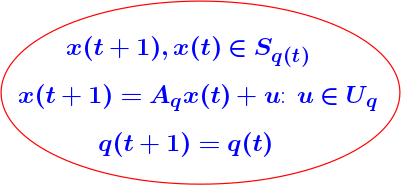
\includegraphics[scale=0.4]{fig/cont-transition.png}
\caption*{{\color{black}\hspace{1em} Continuous transition}}
\end{figure}
\end{minipage}
\hspace{1em}\vrule\hspace{1em}
\begin{minipage}{0.45\textwidth}
\begin{figure}
\centering
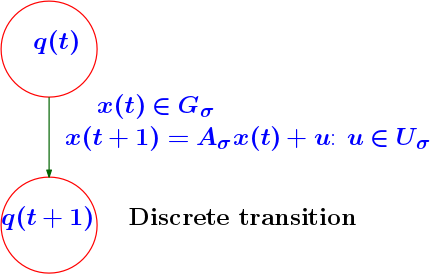
\includegraphics[scale=0.35]{fig/dis-transition.png}
\end{figure}
\end{minipage}
\end{frame}

\begin{frame}{Positive Invariant}
\begin{overprint}
\only<1>{
\begin{figure}
\center
\caption*{{\large \eqncol{$P$: Positive Invariant $\Leftrightarrow$ $\forall x(t)\in P:~ x(t+1)\in P$}}}
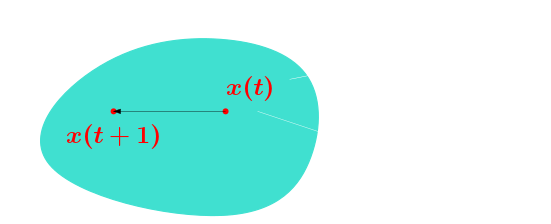
\includegraphics[scale=0.4]{fig/PosInv1.png}
\end{figure}
}
\only<2>{
\begin{figure}
\center
\caption*{{\large \eqncol{$P$: Positive Invariant $\Leftrightarrow$ $\forall x(t)\in P:~ x(t+1)\in P$}}}
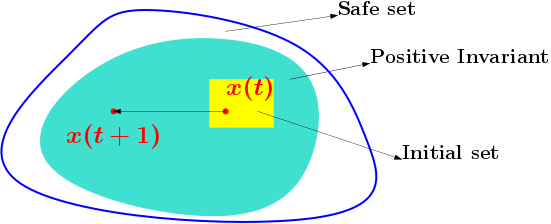
\includegraphics[scale=0.4]{fig/PosInv.png}
\end{figure}
}
\pause
\begin{itemize}
\item (\textcol{Initial set} \eqncol{$\subseteq$} \textcol{Positive Invariant} \eqncol{$\subseteq$} \textcol{Safe Set}) \eqncol{$\Leftrightarrow$} \textcol{System is safe}.
\item Useful for \textcol{Proving Safety Properties}, finding \textcol{ Safe Initial Conditions}.
\end{itemize}
\end{overprint}
\end{frame}

\begin{frame}{Set Representations for Computing Positive Invariants}
\begin{itemize}
\item Computing {\color{red} Smallest Positive Invariant} involves {\color{red}Iterative computations} $\Rightarrow$ {\color{red}Convergence can be very Slow}\pause
\item Use \textcol{Specific set representations} to \textcol{Accelerate convergence}.\\
{\color{brown} Examples}
\begin{enumerate}
\item \textcol{Polytopes} $\Rightarrow$ Use \textcol{Convex Hull} overapproximation~\cite{todo}.
\item \textcol{Ellipsoids} $\Rightarrow$ solve \textcol{Linear Matrix Inequalities}.
\item \textcol{Template Linear inequalities} \cite{todo} and \textcol{Quadratic Inequalities} \cite{todo} \\$\Rightarrow$ Use \textcol{ Widening} or \textcol{Policy Iteration}.
\end{enumerate}
\end{itemize}
\end{frame}
































\bibliography{ref}



\end{document}
